\documentclass[a4paper]{article}

\usepackage[pages=all, color=black, position={current page.south}, placement=bottom, scale=1, opacity=1, vshift=5mm]{background}
%\SetBgContents{
%	\tt This work is shared under a \href{https://creativecommons.org/licenses/by-sa/4.0/}{CC BY-SA 4.0 license} unless otherwise noted
%}      % copyright

\usepackage[margin=1in]{geometry} % full-width

% AMS Packages
\usepackage{amsmath}
\usepackage{amsthm}
\usepackage{amssymb}

% Unicode
\usepackage[utf8]{inputenc}
\usepackage{hyperref}
\hypersetup{
	unicode,
%	colorlinks,
%	breaklinks,
%	urlcolor=cyan,
%	linkcolor=blue,
	pdfauthor={Author One, Author Two, Author Three},
	pdftitle={A simple article template},
	pdfsubject={A simple article template},
	pdfkeywords={article, template, simple},
	pdfproducer={LaTeX},
	pdfcreator={pdflatex}
}

% Natbib
\usepackage[sort&compress,numbers,square]{natbib}
\bibliographystyle{mplainnat}

% Theorem, Lemma, etc
\theoremstyle{plain}
\newtheorem{theorem}{Theorem}
\newtheorem{corollary}[theorem]{Corollary}
\newtheorem{lemma}[theorem]{Lemma}
\newtheorem{claim}{Claim}[theorem]
\newtheorem{axiom}[theorem]{Axiom}
\newtheorem{conjecture}[theorem]{Conjecture}
\newtheorem{fact}[theorem]{Fact}
\newtheorem{hypothesis}[theorem]{Hypothesis}
\newtheorem{assumption}[theorem]{Assumption}
\newtheorem{proposition}[theorem]{Proposition}
\newtheorem{criterion}[theorem]{Criterion}
\theoremstyle{definition}
\newtheorem{definition}[theorem]{Definition}
\newtheorem{example}[theorem]{Example}
\newtheorem{remark}[theorem]{Remark}
\newtheorem{problem}[theorem]{Problem}
\newtheorem{principle}[theorem]{Principle}

\usepackage{graphicx, color}
\graphicspath{{fig/}}

%\usepackage[linesnumbered,ruled,vlined,commentsnumbered]{algorithm2e} % use algorithm2e for typesetting algorithms
\usepackage{algorithm, algpseudocode} % use algorithm and algorithmicx for typesetting algorithms
\usepackage{mathrsfs} % for \mathscr command

%%%%%%%%%%%%%%%%%%%%%%%%%%%%%%%%%%%%%%%%%%%%%%%%%%%%%%%%%%%%%%%%%%%%%%
% Experiment to create a table with arrows between selected pairs of
% cells, copied from:
% https://tex.stackexchange.com/questions/163174/table-with-arrows-between-cells
\usepackage{tabularx}
\usepackage{tikz}
%\tikzset{every picture/.style={remember picture}}

\renewcommand\tabularxcolumn[1]{m{#1}}
\newcolumntype{M}{>{\centering\arraybackslash}m{1cm}}
\newcolumntype{Y}{>{\centering\arraybackslash}X}

\newcommand\tikzmark[2]{%
\tikz[remember picture,baseline] \node[inner sep=2pt,outer sep=0] (#1){#2};%
}

\newcommand\link[2]{%
\begin{tikzpicture}[remember picture, overlay, >=stealth, shift={(0,0)}]
  \draw[->] (#1) to (#2);
\end{tikzpicture}%
}
%%%%%%%%%%%%%%%%%%%%%%%%%%%%%%%%%%%%%%%%%%%%%%%%%%%%%%%%%%%%%%%%%%%%%%

% Author info
\title{Andy's science scratch pad}
\author{J. Andrew Fingerhut (\texttt{andy.fingerhut@gmail.com})}

\date{
        July 18, 2025
%	\today
}

\newcommand{\ihat}{\textbf{i}}
\newcommand{\jhat}{\textbf{j}}
\newcommand{\khat}{\textbf{k}}
\newcommand{\rhat}{\hat{\textbf{r}}}
\newcommand{\vect}[1]{\textbf{#1}}

\begin{document}
\maketitle

%\begin{abstract}
%  abstract here
%\end{abstract}

\tableofcontents

\section{Introduction}
\label{sec:intro}

This document is a place to write up little bits on science.

Some notation:

$\ihat$ is the unit vector from left to right.
$\jhat$ is the unit vector upwards.
$\khat$ is the unit vector pointed out of the page toward the reader.

$\gamma = 1/\sqrt{1-v^2/c^2}$ is the Lorentz factor.


\section{Electromagnetic force between two point charges at rest relative to each other}
\label{sec:twocharges}

Scenario 1: There are two point charges $a$ and $b$ both with charge
$q$ at rest relative to each other at a distance $r$ apart (see
Figure~\ref{fig:two-charges-at-rest}).  They are at rest relative
to us.  In this case they both experience a force directly away from
the other due to electric repulsion.  There is no magnetic force, as
both charges are at rest so there are no magnetic fields.

\begin{figure}[ht]
	\centering
	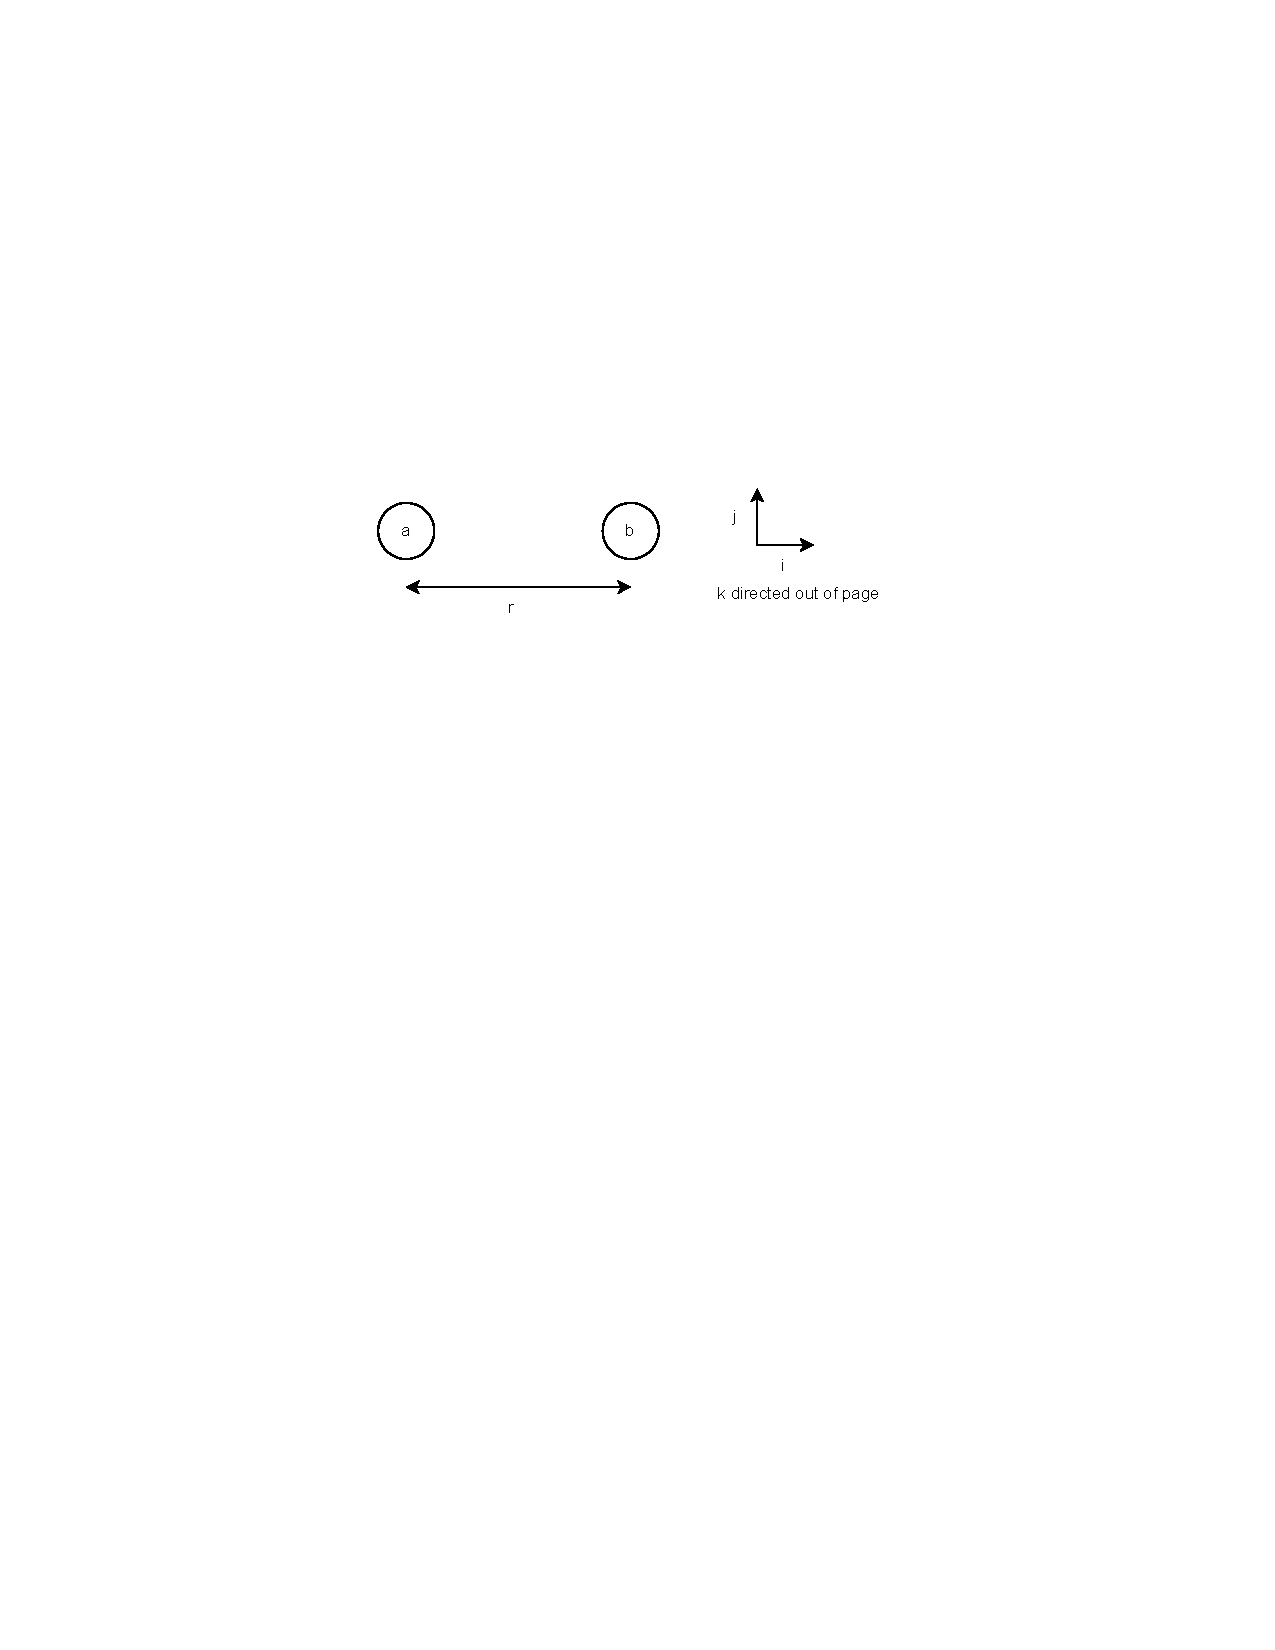
\includegraphics[width=0.6\textwidth]{two-charges-at-rest-cropped.pdf}
	\caption{Two point charges at rest}
	\label{fig:two-charges-at-rest}
\end{figure}


Scenario 2: The same as scenario 1, but both charges are moving with
constant velocity $v$ in the upwards direction (see
Figure~\ref{fig:two-charges-moving}).  Since they are moving they
create magnetic fields.

\begin{figure}[ht]
	\centering
	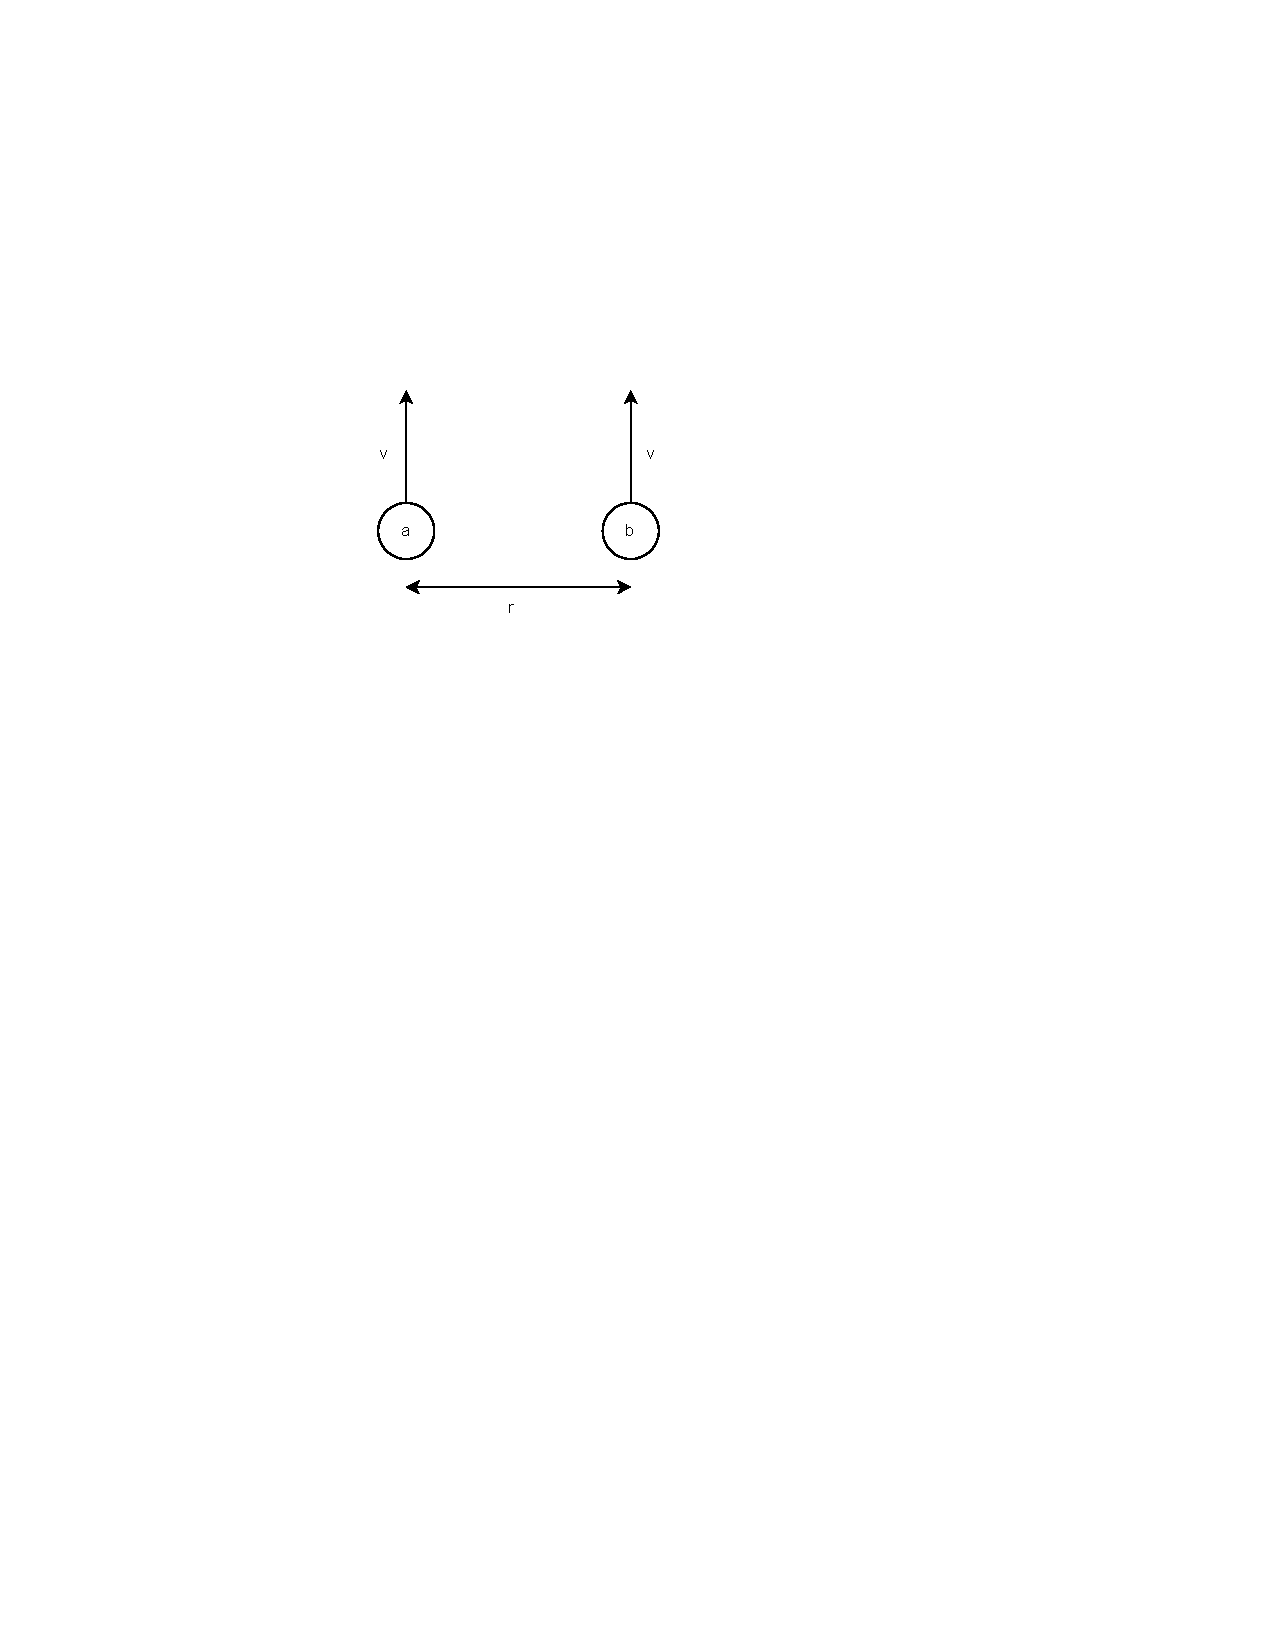
\includegraphics[width=0.4\textwidth]{two-charges-moving-cropped.pdf}
	\caption{Two point charges moving at same constant velocity}
	\label{fig:two-charges-moving}
\end{figure}

Questions:
\begin{itemize}
  \item What is the net force on charge $b$ in each scenario?
  \item Is it the same in both scenarios, or different?
  \item Why?
\end{itemize}


\subsection{Scenario 1: Both charges at rest}

As mentioned before, there is no current or motion of any charges in
this scenario, so no magnetic fields.  The electric repulsion force on
charge $b$ is easily calculated from Coulomb's Law~\cite{CoulombsLaw}.
Charge $b$ is to the right of charge $a$, so the direction of the force is
$\ihat$, away from charge $a$.

\begin{equation}
\vect{E}_1 = \frac{1}{4 \pi \epsilon_0} \frac{q}{r^2} \ihat \label{eq:E1}
\end{equation}

\begin{equation}
\vect{B}_1 = 0
\end{equation}

\begin{equation}
\vect{F}_1 = q(\vect{E}_1 + \vect{v} \times \vect{B}_1)
           = q \vect{E}_1   \label{eq:F1}
\end{equation}


\subsection{Scenario 2: Both charges with equal and constant velocity upwards}

\subsubsection{Scenario 2 calculated by electromagnetic field equations from Griffiths}

The Wikipedia page on the Biot-Savart
Law~\cite{EMFieldFromPointCharge} has a subsection titled ``Point
charge at constant velocity'' that says:

\begin{quote}
the Biot–Savart law applies only to steady currents and a point charge
moving in space does not constitute a steady current
\end{quote}

I will thus use the equations in that section to calculate the
electric and magnetic fields here.  The relevant parts of the
Wikipedia page are copied below.

\begin{quote}
In the case of a point charged particle $q$ moving at a constant
veclocity $\vect{v}$, Maxwell's equations give the following
expression for the electric field and magnetic field:
\end{quote}
\begin{align}
\vect{E} & = \frac{q}{4 \pi \epsilon_0} \frac{1-\beta^2}{(1-\beta^2 \sin^2 \theta)^{3/2}} \frac{{\rhat}'}{|r'|^2} \label{eq:EforPtChg} \\
\vect{B} & = \frac{1}{c^2} \vect{v} \times \vect{E} \label{eq:BforPtChg}
\end{align}
where:
\begin{itemize}
    \item ${\rhat}'$ is the unit vector pointing from the current
      (non-retarded) position of the particle to the point at which
      the field is being measured,
    \item $\beta = v/c$ is the speed in units of $c$, and
    \item $\theta$ is the angle between $\vect{v}$ and ${\rhat}'$.
\end{itemize}

The equations above appear to be identical to equations (10.75) and
(10.76) in Griffiths~\cite{Griffiths1998}.  Griffiths comments on the formula for the electric field:

\begin{quote}
Notice that $\vect{E}$ points along the line from the {\em present}
position of the particle.  This is an extraordinary coincidence, since
the ``message'' came from the retarded position.  Because of the
$\sin^2 \theta$ in the denominator, the field of a fast-moving charge
is flattened out like a pancake in the direction perpendicular to the
motion (Fig. 10.10).  In the forward and backward directions
$\vect{E}$ is reduced by a factor $(1 - v^2/c^2)$ relative to the
field of a charge at rest; in the perpendicular direction it is
{\em enhanced} by a factor $1 / \sqrt{ 1 - v^2/c^2}$.
\end{quote}

Calculation: To get the force on charge $b$, we first calculate the
$\vect{E}$ and $\vect{B}$ fields at the position of charge $b$.

Charge $b$ is directly to the right of charge $a$, so ${\rhat}' = \ihat$
and $\theta = 90^{\circ}$.

\begin{align}
\vect{E}_2
  & = \frac{q}{4 \pi \epsilon_0} \frac{1-\beta^2}{(1-\beta^2 \sin^2 \theta)^{3/2}} \frac{{\rhat}'}{|r'|^2} & & \text{${\rhat}' = \ihat$, $|r'| = r$, $\theta=90^{\circ}$, simplify fraction} \nonumber \\
  & = \frac{q}{4 \pi \epsilon_0} \frac{1}{(1-\beta^2)^{1/2}} \frac{\ihat}{r^2} & & \text{part of this is $\gamma$, by~\eqref{eq:E1} the rest is $\vect{E}_1$} \nonumber \\
  & = \gamma \vect{E}_1 \label{eq:E2value}
\end{align}

Note that $\vect{E}_2$ being $\gamma$ times larger than $\vect{E}_1$
is consistent with the comment from Griffiths above: ``in the
perpendicular direction it ($\vect{E}$) is {\em enhanced} by a factor
$1 / \sqrt{ 1 - v^2/c^2}$''.

\begin{align*}
\vect{F}_2
  & = q (\vect{E}_2 + \vect{v} \times \vect{B}_2)   & & \text{replace $\vect{B}_2$ with \eqref{eq:BforPtChg}} \\
  & = q (\vect{E}_2 + \vect{v} \times (\frac{1}{c^2} \vect{v} \times \vect{E}_2))  & & \vect{v} \times \vect{E}_2 = - v E_2 \khat \\
  & = q (\vect{E}_2 - \frac{v E_2}{c^2} \vect{v} \times \khat)  & & \vect{v} \times \khat = v \ihat \\
  & = q (\vect{E}_2 - \frac{v^2 E_2}{c^2} \ihat) \\
  & = q (1 - \frac{v^2}{c^2}) \vect{E}_2 \\
  & = \frac{q \vect{E}_2}{\gamma^2} & & \text{by~\eqref{eq:E2value} \ } \vect{E}_2 = \gamma \vect{E}_1 \\
  & = \frac{q \vect{E}_1}{\gamma} & & \text{by~\eqref{eq:F1} \ } \vect{F}_1 = q \vect{E}_1 \\
  & = \frac{\vect{F}_1}{\gamma}
\end{align*}

Thus $\vect{F}_2$ differs from $\vect{F}_1$ by a factor of $\gamma$.

TODO: Why?

I do not know how to check the answer below, but it appears that three
of the answers to an on-line question similar to
mine~\cite{PhysicsSEIsLorentzForceFrameIndependent} say that the
Lorentz force formula $\vect{F} = q(\vect{E} + \vect{v} \times
\vect{B})$ is {\em not} invariant in all inertial frames, but perhaps
a slightly modified version of that formula is invariant between
different inertial frames.  I quote one such answer below:

\begin{quote}
Just for completeness if permitted: Following Section 3.1 from the
book ``Gravitation'' of Misner, Thorne, and Wheeler the truly (at all
speeds) frame independent force is $\frac{dP}{d \tau} = \gamma (E + v
\times B)$ (in fact this is only the spacial component of the four
force).  $\tau$ is proper time and $\gamma$ the well-known Lorentz
Factor. -- Kurt G. Aug 28, 2021
\end{quote}


\subsubsection{Scenario 2 calculated by Heaviside-Feynman formula}

The Wikipedia page on Jefimenko's Equations~\cite{JefimenkosEquations}
has a subsection titled ``Heaviside-Feynman formula'' that gives
equations for the electric and magnetic field at a point due to a
single moving point charge.

\begin{align}
\vect{E} & = \frac{-q}{4 \pi \epsilon_0}
             \left[
               \frac{\vect{e}_{r'}}{r'^2}
               + \frac{r'}{c} \frac{d}{dt} \left( \frac{\vect{e}_{r'}}{r'^2} \right)
               + \frac{1}{c^2} \frac{d^2}{dt^2} \vect{e}_{r'}
             \right]
             \label{eq:HF-EforPtChg} \\
\vect{B} & = - \vect{e}_{r'} \times \frac{\vect{E}}{c}
             \label{eq:HF-BforPtChg}
\end{align}

Here $\vect{e}_{r'}$ is a unit vector pointing from the observer to
the charge and $r'$ is the distance between observer and charge.
Since the electromagnetic field propagates at the speed of light, both
of these quantities are evaluated at the retarted time $t - r'/c$.

I believe ``observer'' above means ``the position for which we are
calculating $E$ and $B$ fields''.

Assume here that the point charges are kept at distance $r$ apart from
each other, always horizontally, e.g. because they are connected by a
stiff insulating rod.  This simplifies our job of calculating $E$,
because then $\vect{e}_{r'}$ and $r'$ are unchanging over time, and
their derivates are thus 0.

We want to calculate $r'$ as the vector from the position of charge
$b$ to the position where charge $a$ was when it emitted an electric
field propagated at speed $c$ to $b$.  See
Figure~\ref{fig:retarded-position}.

\begin{figure}[ht]
	\centering
	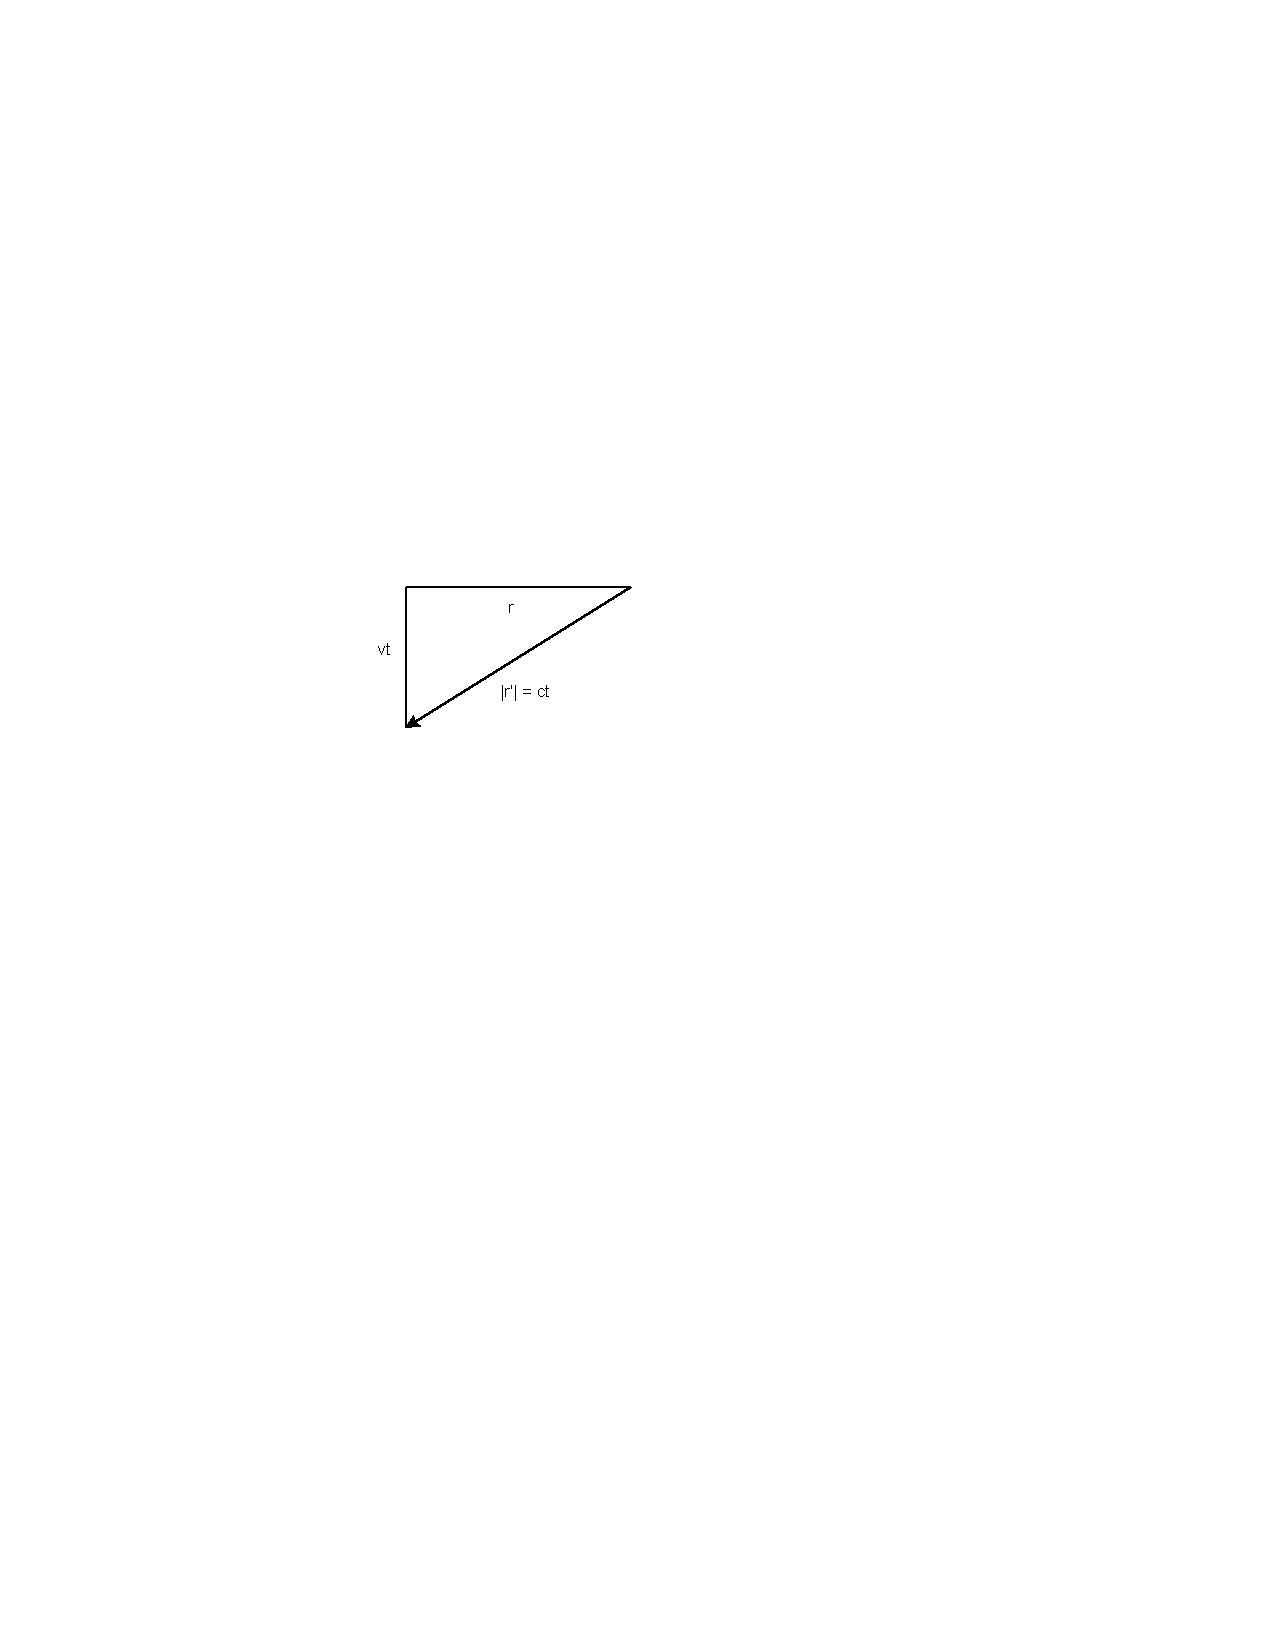
\includegraphics[width=0.5\textwidth]{retarded-position-cropped.pdf}
	\caption{The retarded position of charge $a$ from charge $b$}
	\label{fig:retarded-position}
\end{figure}

Solve for $t$ using Pythagorean theorem since $r$ and $v$ are known
constants:
\begin{align*}
r^2 + (vt)^2 & = (ct)^2 \\
t^2 (c^2 - v^2) & = r^2 \\
t^2 & = \frac{r^2}{c^2 - v^2} \\
t & = \frac{r}{\sqrt{c^2-v^2}} \\
  & = \frac{r}{c \sqrt{1 - v^2/c^2}} \\
  & = \gamma r / c
\end{align*}

This gives us $r' = ct = \gamma r$, and $\vect{e}_{r'}$ is:

\begin{align*}
\vect{e}_{r'} & = \frac{-r \ihat - (\gamma r v / c) \jhat}{\gamma r} \\
  & = - \frac{1}{\gamma} \ihat - \frac{v}{c} \jhat
\end{align*}

Plugging in this value for $\vect{e}_{r'}$ into
Equation~\eqref{eq:HF-EforPtChg} gives:

\begin{align*}
\vect{E}_3 & = \frac{q}{4 \pi \epsilon_0}
             \left[
               \frac{\frac{1}{\gamma} \ihat + \frac{v}{c} \jhat}{\gamma^2 r^2}
             \right]
\end{align*}

Note that $\vect{E}_3$ is parallel to $\vect{e}_{r'}$, thus
$\vect{B}_3$ from Equation~\eqref{eq:HF-BforPtChg} is 0.

This gives the force on charge $b$ as:
\begin{align*}
\vect{F}_3
  & = q (\vect{E}_3 + \vect{v} \times \vect{B}_3) \\
  & = q \vect{E}_3
\end{align*}
The direction of $\vect{F}_3$ is different than $\vect{F}_1$ and $\vect{F}_2$.
Below is the relative magnitude of $\vect{E}_3$ to $\vect{E}_1$:
\begin{align*}
E_3 & = \frac{1}{\gamma^2} E_1 \\
F_3 & = \frac{1}{\gamma^2} F_1
\end{align*}

TODO: It seems {\em very} odd to me that $\vect{B}_3 = 0$.

After Feynman explains what the retarded direction and distance
$\vect{r'}$ is, he says~\cite{FeynmanLecturesVolICh28}:
\begin{quote}
That would be easy enough to understand, too, but it is also
wrong.  The whole thing is much more complicated.
\end{quote}
Unfortunately there are no footnotes or citation to explain what he
meant by this.


\section{Simple scenarios in special relativity and Lorentz Ether Theory}
\label{sec:sr}

Definitions of some terms:
\begin{align}
  \beta & = v / c \label{defn:betaB} & & \text{the {\em relativistic velocity}, or {\em velocity ratio}} \\
  \gamma & = \frac{1}{\sqrt{1 - \beta^2}} & & \text{the {\em Lorentz factor}} \label{defn:LorentzFactor} \\
  D & = \sqrt{ \frac{1 + \beta}{1 - \beta} } & & \text{the {\em Doppler factor}} \label{defn:DopplerFactor}
\end{align}
Later in this article we typically write a subscript after $v$,
$\beta$, $\gamma$, and $D$ to indicate the entity that has the
relevant velocity $v$.  The context should make it clear in what
inertial frame that velocity $v$ applies.

We will use these definitions in scenarios where $-c < v < c$.
Thus:
\begin{align}
-1 & \leq \beta < 1 \nonumber \\
\gamma & \geq 1 & & \text{$\gamma$ increases as $|\beta|$ does} \nonumber \\
\lim_{\beta \rightarrow 1} \gamma & = +\infty \nonumber \\
\lim_{\beta \rightarrow -1} \gamma & = +\infty \nonumber \\
D & = \gamma (1+\beta) > 0 & & \text{$D$ increases as $\beta$ does} \label{eqn:DaltFormula}
\end{align}


\subsection{Special Relativity Scenario 1: Two entities moving relative to each other at constant velocity}
\label{sec:scen1}

$A$ is at rest.  $B$ is moving at constant velocity $v_B$ relative to $A$,
either directly away from $A$, or directly towards $A$.
$v_B > 0$ means $B$ moves away from $A$.
$v_B < 0$ means $B$ moves towards $A$.


\subsubsection{$B$ sends periodic pulses to $A$}
\label{sec:scen1BtoA}

$B$ uses his local clock to time the sending of radio pulses to $A$,
sending pulses once every time interval $T$.
At what period does $A$ receive the pulses?

Define $q_A(n)$ to be the time on A's clock when the $n$-th pulse is
transmitted by $B$, and $q_B(n)$ to be the time on B's clock when it
transmits the $n$-th pulse.

$q_B(n) = nT$ by the setup of the experiment.

By the assumptions of special relativity, $A$ deduces that $B$'s clock
is running $\gamma_B$ times slower than $A$'s clock.  Note: $A$ cannot
directly observe $B$'s clock, as it is too far away.  From this $A$
also deduces:
\begin{equation}
q_A(n) = \gamma_B nT + \Delta  \label{eqn:scen1timeA}
\end{equation}
$\Delta$ is the time that $A$ reads on his clock
when $B$ reads 0 on his clock.  The value of $\Delta$
is irrelevant to the final result we seek.

$B$'s distance from $A$ at $A$'s time $t_A$ is
$x_B(t_A) = I_B + v_B t_A$.
$I_B > 0$ is $B$'s initial distance from $A$ at $t_A=0$.
The value of $I_B$ is also irrelevant to the final result we seek,
as long as it is large enough that $x_B(t_A) > 0$ remains
true while $B$ emits all of the pulses we consider (two pulses is enough).

Also by the assumptions of special relativity, $A$ deduces that $B$'s
pulse signal will propagate at the one-way speed $c$.  The pulse will
thus take time $x_B(q_A(n))/c$ to propagate to $A$.

$A$'s clock thus shows time $r_A(n) = q_A(n) + x_B(q_A(n))/c$ when the $n$-th
pulse arrives at $A$.  With a little algebra:
\begin{align*}
r_A(n)
  & = q_A(n) + x_B(q_A(n))/c & & \text{definition of $r_A(n)$} \\
  & = q_A(n) + (I_B + v_B q_A(n))/c & & \text{substitute equation for $x_B$} \\
  & = (1 + v_B/c) q_A(n) + I_B/c & & \text{rearrangement by algebra} \\
  & = (1 + \beta_B) (\gamma_B nT + \Delta) + I_B/c & & \text{Defn.~\eqref{defn:betaB} and Eqn.~\eqref{eqn:scen1timeA}} \\
  & = (1 + \beta_B) \gamma_B Tn + ((1 + \beta_B) \Delta + I_B/c) & & \text{algebra to collect all terms independent of $n$ at the end}
\end{align*}
The time that $A$ measures on his clock between two consecutive received
pulses is:
\begin{align*}
r_A(n+1) - r_A(n)
  & = (1 + \beta_B) \gamma_B T & & \text{by calculation of $r_A(n)$ above} \\
  & = D_B T & & \text{Eqn.~\eqref{eqn:DaltFormula}}
\end{align*}
The pulses arrive at $A$ with a period of $D_B T$ measured on $A$'s clock.

Suppose that $A$ knows somehow the period $T$ that $B$ uses as its
period for transmitting pulses, e.g. because they agreed and arranged
this beforehand.  Then $A$ can measure the period between received
pulses on his clock and divide it by $T$ to calculate $D_B$.
By Corollary~\ref{cor:DdeterminesBeta} in
Appendix~\ref{app:DopplerFactor}, $A$ can calculate from $D_B$ the one
value of $\beta_B$ in the range $(-1, 1)$ that corresponds to it, and
$v_B$ in the range $(-c, +c)$.

Note 1: There is {\em nothing} in this derivation that relies upon prior
knowledge of the Doppler factor, or under what conditions it is
applicable.  That expression arose in
the process of calculating the answer, using only the assumptions that
light moves isotropically at speed $c$ in $A$'s frame, and that $A$
can deduce that $B$'s clock is running $\gamma_B$ times slower than
$A$'s clock.


\subsubsection{$A$ sends periodic pulses to $B$}
\label{sec:scen1AtoB}

Now $A$ uses his local clock to time the sending of radio pulses to $B$,
sending pulses once every time interval $T$.
At what period does $B$ receive the pulses?

While we could switch perspectives to $B$'s inertial frame, we will
not.  Instead, we are going to do all of the calculations in $A$'s
inertial frame.

The definitions of Section~\ref{sec:sr} remain the same here, but note
that the values of $q_A(n)$ and $q_B(n)$ here are {\em different} than
those in Section~\ref{sec:scen1BtoA}.

Define $q_A(n) = nT$ to be the time on A's clock when it transmits its
$n$-th pulse.

At all times $t_A$, $B$ is a distance $x_B(t_A) = I_B + v_B t_A$ away from $A$.
As in the previous section, $I_B > 0$ is any value large enough
that $x_B(t_A)$ remains positive while $A$ emits all of the pulses we consider.

$A$ assumes by special relativity that its pulse propagates with one-way
speed $c$ to $B$.  The pulse's position at time $t_A \geq q_A(n)$ is
$c(t_A - q_A(n))$.

On $A$'s clock, $A$ deduces that
its $n$-th pulse catches up to $B$ at a time $r_A(n)$ that satisfies the equation:
\begin{align}
x_B(r_A(n)) & = c(r_A(n) - q_A(n)) & & \text{$B$'s position equals light pulse's position} \nonumber \\
I_B + v_B r_A(n) & = c(r_A(n) - nT) & & \text{substitute for defns. of $x_B$ and $q_A(n)$} \\
I_B/c + (v_B/c) r_A(n) & = r_A(n) - nT & & \text{divide by $c$} \nonumber \\
nT + I_B/c & = (1 - v_B/c) r_A(n) & & \text{a little more algebra} \nonumber \\
r_A(n) & = \frac{nT}{1 - v_B/c} + \frac{I_B}{c-v_B} & & \text{divide by $(1-v_B/c)$} \nonumber \\
r_A(n) & = \frac{nT}{1 - \beta_B} + \frac{I_B}{c-v_B} & & \text{Defn.\eqref{defn:betaB}} \label{eqn:scen1Arecvtime}
\end{align}
By the assumptions of special relativity, $A$ deduces that $B$'s clock
is running $\gamma_B$ times slower than $A$'s clock.
Thus $B$'s time when receiving the $n$-th pulse is
the following, where $\Delta$ is the time that $B$ reads on his clock
when $A$ reads 0 on his clock (as in the previous section,
the value of $\Delta$ is irrelevant in our final answer):
\begin{align*}
r_B(n) & = r_A(n) / \gamma_B + \Delta & & \text{$B$'s clock slower by factor $\gamma_B$} \\
       & = \frac{nT}{\gamma_B(1 - \beta_B)} + (\frac{I_B}{\gamma_B(c-v_B)} + \Delta) & & \text{Eqn.~\eqref{eqn:scen1Arecvtime}, move things independent of $n$ to end}
\end{align*}
The time that $B$ measures on his clock between two consecutive received
pulses is:
\begin{align*}
r_B(n+1) - r_B(n)
  & = \frac{T}{\gamma_B(1 - \beta_B)} & & \text{by calculation of $r_B(n)$ above} \\
  & = \frac{\sqrt{1 - \beta_B^2}}{1 - \beta_B} T & & \text{Defn.~\eqref{defn:LorentzFactor}} \\
  & = \sqrt{ \frac{1 + \beta_B}{1 - \beta_B} } T & & \text{a little algebra} \\
  & = D_B T & & \text{Defn.~\eqref{defn:DopplerFactor}}
\end{align*}
$B$ will observe pulses arriving with period $D_B T$ according to
$B$'s clock.

While this formula for the period between received pulses
is very similar to the one in the previous section, note that
both the sending and receiving period are being measured on different
clocks than there.

As in the previous section, if $B$ somehow knows $T$,
he can measure the interal between receive pulses,
divide it by $T$ to calculate $D_B$,
then use that to calculate $\beta_B$ and $v_B$.


\subsubsection{Relationship to Lorentz Ether Theory}
\label{sec:scen1LET}

Note in Sections~\ref{sec:scen1BtoA} and~\ref{sec:scen1AtoB}, that
except for algebra and the definitions of symbols from
Section~\ref{sec:sr}, the only assumptions we used from special relativity were:
\begin{itemize}
\item The one-way speed of light is $c$ in all directions in $A$'s
  inertial frame.
\item In $A$'s frame, $B$'s clock runs at a slower rate, by a factor
  of $1/\gamma_B$, relative to $A$'s clock.
\end{itemize}
By Lorentz Ether Theory, suppose that somehow we know that $A$ is at
rest relative to the ether, then:
\begin{itemize}
\item The one-way speed of light is $c$ in all directions relative to
  the ether, and thus also relative to $A$.
\item $B$ is moving at velocity $v_B$ relative to the ether, and thus
  $B$'s clock physically runs at a slower rate, $1/\gamma_B$ times as
  fast as the true time.  $A$'s clock runs at the full rate of true
  time, the same as any other clocks at rest relative to the ether.
\end{itemize}

TODO: Find a way to explain the following better.

I had heard from a not-yet-in-depth learning about special relativity
that when $A$ and $B$ are moving at constant velocity towards or away
from each other, that $A$ observed that $B$'s clock ran slower by a
factor of $\gamma$, and $B$ observed that $A$'s clock ran slower by a
factor of $\gamma$.  (Note: I do not claim that those are fully
precise statements, but there is definitely a sense in which special
relativity does say something similar to this.)

In $A$'s frame observing $B$'s clock run slower, that seems perfectly
consistent with Lorentz Ether Theory's statement that if $A$ is at
rest relative to the ether, and $B$ moves at constant velocity $v_B$
relative to the ether, that $B$ experiences duration dilation,
i.e. its clock physically runs slower than $A$'s by a factor of
$\gamma_B$.  In this situation $A$'s clock runs at full speed,
i.e. $\gamma_B$ times {\em faster} than $B$'s.

But what about Lorentz Ether Theory's position on the converse
statement?  That is, from $B$'s point of view, does $B$ observe $A$'s
clock running $\gamma_B$ times slower?  If so, how can that possibly
make sense?

I now believe that the answer is that the statements in special
relativity can be made a bit more precise by saying something like
this: Because $A$ is following special relativity's assumptions,
i.e. in $A$'s frame the speed of light propagates isotropically at
constant speed $c$, therefore $A$ can deduce that any clocks moving at
constant speed $v$ directly towards or away from $A$ run $\gamma$
times slower, and make further calculations from that deduction.

$A$ does not actually {\em observe} such clocks directly over any
appreciable interval of time, so they are always, or almost always, so
far away that $A$ cannot make {\em any} direct observations of how
fast such clocks are running.  By ``direct'' observations I mean
``with light propagation delay very close to 0 between $A$ and the
entity being observed''.

Suppose in some future context of knowledge that not only is Lorentz
Ether Theory proven, but in such a way that we know how to measure our
speed relative to the ether.

Then, in the scanario described, we would know that $A$'s clock is
running at full speed, and light propagates isotropically at constant
speed $c$ relative to the ether, and thus also relative to $A$.

Everyone with this knowledge would be able to deduce that $B$'s clock
is running $\gamma$ times slower than full speed.  Also, that
$A$'s clock is running $\gamma$ times {\em faster} than $B$'s clock
(and that all of $A$'s local physical processes are proceeding
$\gamma$ times faster than similar local physical processes of $B$).

Further, light does {\em not} propagate at the same speed in all
directions relative to $B$.  It does so only with respect to the
ether.

We could also prove that if one chose to make calculations using
special relativity's assumptions in $B$'s frame, one would get the
same answers to these calculations that you do when using Lorentz
Ether Theory.

A hint of corroboration can be seen in the Wikipedia page on time
dilation, which says in the introduction~\cite{WikipediaTimeDilation}:
\begin{quote}
The dilation compares ``wristwatch'' clock readings between events
measured in different inertial frames and is not observed by visual
comparison of clocks across moving frames.
\end{quote}

It seems that any statement similar to:
\begin{itemize}
\item $A$ observes $B$'s clock running slower than their own.
\end{itemize}
could be said in much more detail as either of the following:
\begin{itemize}
\item In accordance with special relativity's time synchronization
  convention that light propagates in $A$'s inertial frame
  isotropically with speed $c$, $A$ deduces that $B$'s clock runs
  slower than $A$'s.
\item $A$ deduces, using the postulate that light moves isotropically
  at speed $c$, that $B$’s clock runs slower, and can then make
  further consistent calculations based on this deduction.
\end{itemize}
And you can swap $A$ and $B$ in that statement.  Without defining new
precise terminology, a shorter precise statement would perhaps be:
\begin{itemize}
\item According to SR, in $A$'s inertial frame we deduce that $B$'s
  clock runs slower.
\end{itemize}


\subsection{Special Relativity Scenario 2: Three entities, two of them moving at constant velocity}
\label{sec:scen2}

$A$ is at rest.
$B$ is moving at constant velocity $v_B$ relative to $A$,
which is away from $A$ if $v_B > 0$, or towards $A$ if $v_B < 0$.
$C$ is moving at constant velocity $v_C$ relative to $A$,
with same sign conventions as $B$'s velocity.

For $B$ sending periodic pulses to $A$ or vice versa, everything in
Sections~\ref{sec:scen1BtoA} and~\ref{sec:scen1AtoB} applies without
change.
For $C$ sending periodic pulses to $A$ or vice versa, everything in
Section~\ref{sec:scen1BtoA} and~\ref{sec:scen1AtoB} applies,
except replace $B$ subscripts
with $C$ subscripts, i.e. use $v_C$, $\gamma_C$, $\beta_C$, and $D_C$.

So it is only pulses between $B$ and $C$ that might present something
new here.

Our calculations in the following sections for pulse signals between
$B$ and $C$ assume that throughout the entire duration of sending and
receiving the pulses of interest, $B$'s position according to its $x$
coordinate is always less than $C$'s $x$ coordinate.  If that
condition is ever violated because $B$ crosses paths with $C$, the
results presented here are no longer applicable after that occurs.  We
use $I_B$ and $I_C$ to represent their initial distances from $A$, and
require that these positions, combined with their velocities, will
ensure this.


\subsubsection{$B$ sends periodic pulses to $C$}
\label{sec:scen2BtoCLETfriendly}

$B$ uses his local clock to time the sending of radio pulses to $C$,
sending pulses once every time interval $T$, according to $B$'s clock.
At what period does $C$ receive the pulses?

To make the calculations as easily applicable to Lorentz Ether Theory
as possible, all calculations will be done in $A$'s inertial frame.

Define $q_A(n)$ and $q_B(n)$ the same way as they were in
Section~\ref{sec:scen1BtoA}.  As explained there, when $A$ makes the
assumptions according to special relativity theory:
\begin{align}
q_B(n) & = nT & & \text{by the setup of the experiment} \nonumber \\
t_A & = \gamma_B t_B + \Delta_B & & \text{$B$'s clock runs $\gamma_B$ times slower than $A$'s} \nonumber \\
q_A(n) & = \gamma_B nT + \Delta_B \label{eqn:scen2timeArelB} \\
t_A & = \gamma_C t_C + \Delta_C & & \text{$C$'s clock runs $\gamma_C$ times slower than $A$'s} \nonumber \\
t_C & = t_A/\gamma_C - \Delta_C/\gamma_C & & \text{equivalent to previous equation, but solved for $t_C$} \label{eqn:scen2timeArelC} \\
x_B(t_A) & = I_B + v_B t_A & & \text{relationship of $B$'s position and time, in $A$'s frame} \label{eqn:scen2posB} \\
x_C(t_A) & = I_C + v_C t_A & & \text{relationship of $C$'s position and time, in $A$'s frame} \label{eqn:scen2posC}
\end{align}
Also by special relativity assumptions, $A$ considers the pulse to
travel from $B$ to $C$ at constant speed $c$.
The $n$-th pulse is emitted at time $q_A(n)$ in $A$'s frame,
so its position as a function of $A$'s time $t_A$ is:
\begin{align*}
l_A(n, t_A)
  & = \text{position of $B$ when emitted} \\
  &   + \text{distance traveled after emission} \\
  & = x_B(q_A(n)) + (t_A - q_A(n)) c & & \text{for any time $t_A \geq q_A(n)$} \\
  & = I_B + v_B q_A(n) + (t_A - q_A(n)) c & & \text{substitute Eqn.~\eqref{eqn:scen2posB}} \\
  & = (v_B - c) q_A(n) + t_A c + I_B & & \text{algebra} \\
  & = (v_B - c) \gamma_B nT + t_A c + ((v_B-c)\Delta_B + I_B) & & \text{substitute Eqn.~\eqref{eqn:scen2timeArelB}} \\
  & = (v_B - c) \gamma_B nT + t_A c + Z & & \text{$Z$ is constants, independent of $n$ and $t_A$}
\end{align*}
To find $A$'s time $r_A(n)$ when $C$ receives the pulse,
solve for the time that makes the pulse position the same as $C$'s position:
\begin{align*}
x_C(r_A(n)) & = l_A(n, r_A(n)) \\
I_C + v_C r_A(n) & = (v_B - c) \gamma_B nT + r_A(n) c + Z & & \text{substitute Eqn.~\eqref{eqn:scen2posC}} \\
(v_C - c) r_A(n) & = (v_B - c) \gamma_B nT + (Z - I_C) & & \text{algebra} \\
r_A(n) & = \frac{v_B - c}{v_C - c} \gamma_B nT + \frac{Z - I_C}{v_C - c} & & \text{divide by $v_C-c$} \\
r_A(n) & = \frac{1 - \beta_B}{1 - \beta_C} \gamma_B nT + \frac{Z - I_C}{v_C - c} & & \text{defn. of $\beta_B, \beta_C$} \\
r_A(n) & = \frac{1 - \beta_B}{1 - \beta_C} \gamma_B nT + Y & & \text{$Y$ is a constant, independent of $n$}
\end{align*}
According to $A$ and its special relativity assumptions,
$C$'s clock runs slower, at a rate $1/\gamma_C$ times that of $A$'s clock.
So $C$'s time $r_C(n)$ to receive the $n$-th pulse sent by $B$ is:
\begin{align*}
r_C(n) & = \frac{1}{\gamma_C} r_A(n) - \Delta_C/\gamma_C & & \text{Eqn.~\eqref{eqn:scen2timeArelC}} \\
       & = \frac{\gamma_B}{\gamma_C} \left( \frac{1-\beta_B}{1-\beta_C} \right) nT + \frac{Y-\Delta_C}{\gamma_C}
\end{align*}
The time that $B$ measures on his clock between two consecutive received
pulses is:
\begin{align*}
r_C(n+1) - r_C(n)
  & = \frac{\gamma_B}{\gamma_C} \left( \frac{1-\beta_B}{1-\beta_C} \right) T \\
  & = \sqrt{ \frac{1-\beta_C^2}{1-\beta_B^2} } \left( \frac{1-\beta_B}{1-\beta_C} \right) T & & \text{Defn.~\eqref{defn:LorentzFactor}} \\
  & = \sqrt{ \frac{1+\beta_C}{1-\beta_C} } \sqrt { \frac{1-\beta_B}{1+\beta_B} } T & & \text{algebra} \\
  & = ( D_C / D_B ) T & & \text{defn. of $D_B, D_C$}
\end{align*}
So when $B$ sends pulses with period $T$ according to $B$'s clock, $C$
receives from $B$ pulses with period $(D_C / D_B) T$ on $C$'s clock.

Since $D > 0$ and it increases with $\beta$ (see
Appendix~\ref{app:DopplerFactor}), and thus also with $v$:
\begin{itemize}
\item If $v_c > v_B$, then $C$ and $B$ are moving away relative to
  each other, and $D_C > D_B$, thus $(D_C / D_B) > 1$.
\item If $v_c < v_B$, then $C$ and $B$ are getting closer over time,
  and $D_C < D_B$, thus $(D_C / D_B) < 1$.
\end{itemize}

Aside: If you are curious, the answer provided by ChatGPT for solving
this problem can be found in Appendix~\ref{sec:scen2BtoCdoublecheck}.

Near the end of Sections~\ref{sec:scen1BtoA} and~\ref{sec:scen1AtoB},
we noted that if the receiver knew somehow the period $T$ that the
sender is sending pulses, the receiver could calculate a $D$ value
that enabled the receiver to determine what the velocity of $B$ is.

In the current scenario, the receiver $C$, if it knows $T$, can
measure the time interval between pulses it receives, divide by $T$,
and calculate $(D_C / D_B)$.

Thus, with the measurement of the interval between received pulses,
given any two of $T$, $v_A$, and $v_B$, $C$ can calculate the other
one of those (and given values for two of those quantities, there is
only one value possible for the remaining one).
But from the measurement of the interval between received pulses and
$T$, that is not enough information for $C$ to calculate either one of
$v_B$ or $v_C$.

However, it {\em can} do the following.  Define $D_r = (D_C / D_B)$.
From Corollary~\ref{thm:velSubLeadsToDopplerFQuotient} in
Appendix~\ref{app:DopplerFactor}, we know that if
$\beta_r = \beta_C \ominus \beta_B$ for some $\beta_C, \beta_B$ values
in the range $(-1, +1)$, then $D_r = D_C / D_B$.

TODO: I am fairly certain it is straightforward to prove the converse:
If in this scenario $C$ calculates the value value of $D_r$, then
calculates $\beta_r = (D_r^2-1)/(D_r^2+1)$, then the only possible
pairs of values $\beta_C, \beta_B$ that could have given this
measurement are those satisfying $\beta_r = \beta_C \ominus \beta_B$.
There are an unlimited number of such pairs of values.

This strongly suggests that the receiver can calculate the
{\em relative} velocity between $B$ and $C$, at least in some sense.
I am not sure yet how to explain that further.

Also note that if we follow Lorentz Ether Theory, but we have no
knowledge of how to determine our motion relative to the ether, these
results show that the receiver can, with knowledge of the sender's
period $T$, still calculate this kind of relative velocity described,
which is interesting.


\subsubsection{$C$ sends periodic pulses to $B$}
\label{sec:scen2CtoBLETfriendly}

The derivation is nearly identical to that in
Section~\ref{sec:scen2BtoCLETfriendly}.
Here we only mention a few equations along the way that have
noticeable differences.

The formula $l_A(n,t_A)$ for the position of the $n$-th pulse emitted
by $C$ at $A$'s time $t_A$ is:
\begin{equation}
l_A(n, t_A) = (v_C + c) \gamma_C nT - t_A c + Z'
\end{equation}
$A$'s time when $B$ receives the $n$-th pulse $r_A(n)$ is:
\begin{equation}
r_A(n) = \frac{1 + \beta_C}{1 + \beta_B} \gamma_C nT + Y'
\end{equation}
and $B$'s time when it receives the $n$-th pulse from $C$ is:
\begin{align*}
r_B(n) & = \frac{1}{\gamma_B} r_A(n) + (\text{constants independent of $n$})
\end{align*}
and finally:
\begin{align*}
r_B(n+1) - r_B(n)
       & = ( D_C / D_B ) T
\end{align*}
Thus $B$, after measuring the interval between received pulses, if it
knows $T$ somehow and can calculate $(D_C / D_B)$, can also calculate
the same kind of relative velocity between $B$ and $C$ as described at
the end of the previous section.


\subsection{Summary of results in this section}
\label{sec:summary}

Here is a summary of what we have shown so far.

\begin{itemize}
\item In the scenario of Section~\ref{sec:scen1} where $A$ is at rest,
  and $B$ is moving at velocity $v_B$ relative to $A$ in $A$'s frame
  (negative for velocity towards $A$, positive for velocity away from
  $A$):
  \begin{itemize}
    \item When $B$ sends pulse signals every time period $T$ according
      to $B$'s clock, $A$ measures received pulses every time period
      $D_B T$ according to $A$'s clock.
    \item When $A$ sends pulse signals every time period $T$ according
      to $A$'s clock, $B$ measures received pulses every time period
      $D_B T$ according to $B$'s clock.
  \end{itemize}
\item In the scenario of Section~\ref{sec:scen2} where $A$ is at rest,
  $B$ and $C$ are moving at velocity $v_B$ and $v_C$ relative to $A$
  in $A$'s frame (same sign conventions as above), and the position of
  $C$ is always ``to the right'' of $B$ during the scenario:
  \begin{itemize}
    \item When $B$ sends pulse signals every time period $T$ according
      to $B$'s clock, $C$ measures received pulses every time period
      $(D_C/D_B) T$ according to $C$'s clock.
    \item When $C$ sends pulse signals every time period $T$ according
      to $C$'s clock, $B$ measures received pulses every time period
      $(D_C/D_B) T$ according to $B$'s clock.
  \end{itemize}
\end{itemize}

The table below is another way to summarize the results of Scenario 1.
All formulas for periods have been simplified by using $T=1$, i.e. you
can multiply them all by $T$ to get the original answer derived
earlier.  It also shows how much the previous period is multiplied by
to get the next period in the sequence of steps from the sender to the
receiver.

%%%%%%%%%%%%%%%%%%%%%%%%%%%%%%%%%%%%%%%%%%%%%%%%%%%%%%%%%%%%%%%%%%%%%%
\begin{tabularx}{1.0\textwidth}{|Y|Y|Y|Y|Y|Y|}
\cline{1-6} \\
         & Period measured locally on $A$'s clock & multiply by factor & Period deduced by $A$, on $A$'s clock, at $B$'s location & multiply by factor & Period measured locally on $B$'s clock \\ \cline{1-6}
$A \rightarrow B$ & $1$\tikzmark{ab1r}{} & \tikzmark{ab2l}{}$\frac{1}{1-\beta_B}$\tikzmark{ab2r}{} & \tikzmark{ab3l}{}$\frac{1}{1-\beta_B}$\tikzmark{ab3r}{} & \tikzmark{ab4l}{}$\frac{1}{\gamma_B}$\tikzmark{ab4r}{} & \tikzmark{ab5l}{}$D_B$ \\ \cline{1-6}
$A \leftarrow B$ & $D_B$\tikzmark{ba1r}{} & \tikzmark{ba2l}{}$(1+\beta_B)$\tikzmark{ba2r}{} & \tikzmark{ba3l}{}$\gamma_B$\tikzmark{ba3r}{} & \tikzmark{ba4l}{}$\gamma_B$\tikzmark{ba4r}{} & \tikzmark{ba5l}{}$1$ \\ \cline{1-6}
\end{tabularx}

\link{ab1r}{ab2l}
\link{ab2r}{ab3l}
\link{ab3r}{ab4l}
\link{ab4r}{ab5l}

\link{ba5l}{ba4r}
\link{ba4l}{ba3r}
\link{ba3l}{ba2r}
\link{ba2l}{ba1r}
%%%%%%%%%%%%%%%%%%%%%%%%%%%%%%%%%%%%%%%%%%%%%%%%%%%%%%%%%%%%%%%%%%%%%%

And the table below is another way to summarize the results of
Scenario 2:

%%%%%%%%%%%%%%%%%%%%%%%%%%%%%%%%%%%%%%%%%%%%%%%%%%%%%%%%%%%%%%%%%%%%%%
% I created the table below, with arrows between selected cells, by
% starting with advice on this Q&A page:
% https://tex.stackexchange.com/questions/163174/table-with-arrows-between-cells
%%%%%%%%%%%%%%%%%%%%%%%%%%%%%%%%%%%%%%%%%%%%%%%%%%%%%%%%%%%%%%%%%%%%%%

\begin{tabularx}{1.0\textwidth}{|Y|Y|Y|Y|Y|Y|Y|Y|}
\cline{1-8} \\
         & Period measured locally on $B$'s clock & multiply by factor & Period deduced by $A$, on $A$'s clock, at $B$'s location & multiply by factor & Period deduced by $A$, on $A$'s clock, at $C$'s location & multiply by factor & Period measured locally on $C$'s clock \\ \cline{1-8}
$B \rightarrow C$ & \tikzmark{bc1l}{} 1 \tikzmark{bc1r}{} & \tikzmark{bc2l}{}$\gamma_B$\tikzmark{bc2r}{} & \tikzmark{bc3l}{}$\gamma_B$\tikzmark{bc3r}{} & \tikzmark{bc4l}{}$\frac{1-\beta_B}{1-\beta_C}$\tikzmark{bc4r}{} & \tikzmark{bc5l}{}$\frac{1-\beta_B}{1-\beta_C}\gamma_B$\tikzmark{bc5r}{} & \tikzmark{bc6l}{}$\frac{1}{\gamma_C}$\tikzmark{bc6r}{} & \tikzmark{bc7l}{}$(D_C/D_B)$ \\ \cline{1-8}
$B \leftarrow C$ & $(D_C/D_B)$\tikzmark{cb1r}{} & \tikzmark{cb2l}{}$\frac{1}{\gamma_B}$\tikzmark{cb2r}{} & \tikzmark{cb3l}{}$\frac{1+\beta_C}{1+\beta_B} \gamma_C$\tikzmark{cb3r}{} & \tikzmark{cb4l}{}$\frac{1+\beta_C}{1+\beta_B}$\tikzmark{cb4r}{} & \tikzmark{cb5l}{}$\gamma_C$\tikzmark{cb5r}{} & \tikzmark{cb6l}{}$\gamma_C$\tikzmark{cb6r}{} & \tikzmark{cb7l}{}$1$ \\ \cline{1-8}
\end{tabularx}

\link{bc1r}{bc2l}
\link{bc2r}{bc3l}
\link{bc3r}{bc4l}
\link{bc4r}{bc5l}
\link{bc5r}{bc6l}
\link{bc6r}{bc7l}

\link{cb7l}{cb6r}
\link{cb6l}{cb5r}
\link{cb5l}{cb4r}
\link{cb4l}{cb3r}
\link{cb3l}{cb2r}
\link{cb2l}{cb1r}
%%%%%%%%%%%%%%%%%%%%%%%%%%%%%%%%%%%%%%%%%%%%%%%%%%%%%%%%%%%%%%%%%%%%%%

In every scenarios, all calculations of movement of $B$, $C$, and
pulse signals were done in $A$'s frame.  Only in the first or last
steps did we do any time conversions between clocks running at
different rates.
Thus both special relativity and Lorentz Ether Theory predict the same
measurements.

The equations for the received time intervals all contain one or more
factors of $D$ that are relativistic Doppler factors.  These arose
naturally out of the calculations, not from any prior knowledge of
Doppler factors.  The velocities involved in these Doppler factors are
strongly related to the relative velocity of the sender and the
receiver.

If we adopt Lorentz Ether Theory, but remain ignorant of how to
measure our velocity relative to the ether, Scenario 2's results
strongly suggest a proper understanding of relative velocity.

%\newpage
\bibliography{refs}

\appendix

\section{Miscellaneous math facts}

\subsection{Math facts about relativistic velocity addition and subtraction in one dimension}
\label{app:1drelvelocityadd}

All of the facts here are quite simple to validate.  I write them out
primarily as an aid to thinking about and remembering them, and they
might also be useful to refer to from elsewhere in this document.

Note that this appendix is restricted to proofs of simple mathematical
relationships about the definitions of one-dimensional relativistic
velocity addition and subtraction formulas.  This appendix makes no
claims about the physical meaning of these operations.

I have read that relativistic velocity addition in 3 dimensions is not
associative.  TODO: If I add any discussion of 3-dimensional
relativity examples to this document, it would be nice to give an
example, perhaps in a separate appendix.

In one dimension, though, all velocities of subliminal entities can be
represented by $v$ such that $-c < v < c$, where negative velocities
are in the opposite direction along the line than positive velocities.

The can also be represented as relativistic velocity $\beta = v/c$,
i.e. a fraction of $c$.  These are in the range $-1 < \beta < 1$.

I will use the notation $v \oplus w$ for relativistic velocity
addition.  While I will use the same symbol $\beta_v \oplus \beta_w$
for relativistic velocity addition of relativistic velocity values,
one should be careful to note that the definition of the operator
$\oplus$ is slightly different for these two cases.

\begin{align}
v \oplus w & = \frac{v+w}{1+\frac{vw}{c^2}} \label{defn:reladd1} \\
v \ominus w & = \frac{v-w}{1-\frac{vw}{c^2}} \label{defn:relsub1} \\
\beta_v \oplus \beta_w & = \frac{\beta_v+\beta_w}{1+\beta_v \beta_w} \label{defn:reladd2} \\
\beta_v \ominus \beta_w & = \frac{\beta_v-\beta_w}{1- \beta_v \beta_w} \label{defn:relsub2}
\end{align}

The proofs are only given for the relativistic velocity
formulas~\eqref{defn:reladd2} and~\eqref{defn:relsub2}.  The proofs
for equations~\eqref{defn:reladd1}
and~\eqref{defn:relsub1} are nearly identical.

We will use the symbols $a, b, c$ to represent arbitrary real values
between -1 and 1, to avoid writing $\beta$ with subscripts all over
the place.

\begin{align}
a \oplus b & = b \oplus a & & \text{addition is commutative} \label{defn:reladdcommutative} \\
(a \oplus b) \oplus c & = a \oplus (b \oplus c) & & \text{addition is associative (1-d only, not 3-d!)} \label{defn:1dreladdassociative} \\
a \oplus 0 & = 0 \oplus a = a \\
a \oplus (-b) & = a \ominus b \\
a \ominus (-b) & = a \oplus b \\
0 \ominus b & = -b \\
a \ominus b & = - (b \ominus a)
\end{align}
The following inequalities only hold if $0 < a < 1$ and $0 < b < 1$:
\begin{align}
a \oplus b & > a \label{inequal:reladdposlarger1} \\
a \oplus b & > b \label{inequal:reladdposlarger2} \\
a \oplus b & < a+b \label{inequal:reladdpossmallerthansum}
\end{align}
The following inequality holds for all $-1 < a < 1$ and $-1 < b < 1$:
\begin{align}
-1 < a \oplus b & < 1 \label{inequal:reladdpossmallerthanc}
\end{align}
The last one is only slightly different if we use velocity addition on
normal velocities, i.e. velocities that are not relativistic velocities,
where $-c < v < c$ and $-c < w < c$:
\begin{align}
-c < v \oplus w & < c \label{inequal:reladdpossmallerthanc2}
\end{align}
The inequalities all have examples where the two sides can be very
nearly equal, such as these:
\begin{align*}
0.1 \oplus 0.001 & \approx 0.100989901 > 0.1 \\
0.1 \oplus 0.1 & \approx 0.198019802 < 0.1+0.1 \\
0.99 \oplus 0.99 & \approx 0.999949498 < 1
\end{align*}

Proving most of these is as simple as substituting the definition of
$a \oplus b$ and $a \ominus b$, and a tiny amount of algebra.

Proving associativity~\eqref{defn:1dreladdassociative} is only a
little bit more algebra, but we will do the steps here:
\begin{align*}
(a \oplus b) \oplus c
  & = \frac{\frac{a+b}{1+ab}+c}{1+\left(\frac{a+b}{1+ab}\right)c} & & \text{use Defn.~\eqref{defn:reladd2} twice} \\
  & = \frac{(a+b)+c(1+ab)}{(1+ab)+(a+b)c} & & \text{multiply numerator and denominator by $(1+ab)$} \\
  & = \frac{a+b+c+abc}{1+ab+ac+bc} & & \text{multiply out the terms}
\end{align*}
Similarly:
\begin{align*}
a \oplus (b \oplus c)
  & = \frac{a+\frac{b+c}{1+bc}}{1+a\left(\frac{b+c}{1+bc}\right)} & & \text{use Defn.~\eqref{defn:reladd2} twice} \\
  & = \frac{a(1+bc)+(b+c)}{(1+bc)+a(b+c)} & & \text{multiply numerator and denominator by $(1+bc)$} \\
  & = \frac{a+abc+b+c}{1+bc+ab+ac} & & \text{multiply out the terms}
\end{align*}
The above two final results are easily seen to be equal.

The inequalities are also not difficult to prove, but we will write
out their short proofs.  Recall that these inequalities are true only
for $0 < a < 1$ and $0 < b < 1$.  Similar inequality hold if both $a$
and $b$ are negative.

For the proof of inequality~\eqref{inequal:reladdposlarger1}, recall
that we can multiply or divide both sides of an inequality by the same
positive number, and the resulting inequality is true if and only if
the original one was.  The symbol $\Leftrightarrow$ below means ``if
and only if'', i.e. the expression before is true if and only if the
expression after is true.
\begin{align*}
a < \frac{a+b}{1+ab}
  & \Leftrightarrow a + a^2 b < a+b & & \text{multiply both sides by $1+ab$, which is positive} \\
  & \Leftrightarrow a^2 b < b & & \text{subtract $a$ from both sides} \\
  & \Leftrightarrow a^2 < 1 & & \text{divide both sides by $b$, which is positive}
\end{align*}
The last inequality is true because $a < 1$.
The proof of inequality~\eqref{inequal:reladdposlarger2} is the same
as above.

To prove $a \oplus b < a+b$
(inequality~\eqref{inequal:reladdpossmallerthansum}):
\begin{align*}
\frac{a+b}{1+ab} < a+b
  & \Leftrightarrow a+b < (a+b)(1+ab) & & \text{multiply both sides by $1+ab$, which is positive} \\
  & \Leftrightarrow 1 < (1+ab) & & \text{divide both sides by $a+b$, which is positive} \\
  & \Leftrightarrow 0 < ab & & \text{subtract 1 from both sides}
\end{align*}
The final inequality is true because both $a$ and $b$ are positive.

Now to prove $a \oplus b < 1$ (part of
inequality~\eqref{inequal:reladdpossmallerthanc}), but recall now we
are doing so for the more general case of all values $-1 < a < 1$ and
$-1 < b < 1$:
\begin{align*}
\frac{a+b}{1+ab} < 1
  & \Leftrightarrow a+b < 1+ab & & \text{multiply both sides by $1+ab$, which is positive} \\
  & \Leftrightarrow b-ab < 1-a & & \text{subtract $a+ab$ from both sides} \\
  & \Leftrightarrow b(1-a) < 1-a & & \text{algebra} \\
  & \Leftrightarrow b < 1 & & \text{divide both sides by $1-a$, which is positive}
\end{align*}
And the last inequality is true.  Proving the part that

\begin{align*}
-1 < \frac{a+b}{1+ab}
  & \Leftrightarrow -(1+ab) < a+b & & \text{multiply both sides by $1+ab$, which is positive} \\
  & \Leftrightarrow -(1+a) < b+ab & & \text{add $ab-a$ to both sides} \\
  & \Leftrightarrow -(1+a) < b(1+a) & & \text{algebra} \\
  & \Leftrightarrow -1 < b & & \text{divide both sides by $1+a$, which is positive}
\end{align*}
And the last inequality is true.


\subsection{Math facts about the Doppler factor}
\label{app:DopplerFactor}

This appendix is restricted to proofs of mathematical relationships.
It makes no claims about the physical meaning of the equations
involved.

Define $D$ as given by Definition~\eqref{defn:DopplerFactor}, repeated
here:
\begin{align*}
D & = \sqrt{ \frac{1 + \beta}{1 - \beta} } & & \text{Repeat of Defn.~\eqref{defn:DopplerFactor}}
\end{align*}
Define it over the entire domain $-1 < \beta < 1$.
\begin{itemize}
\item $D$ approaches 0 as $\beta$ approaches -1.
\item $D$ approaches $+\infty$ as $\beta$ approaches 1.
\item $D$ is an increasing function of $\beta$.
\end{itemize}
The last fact is straightforward to confirm by taking the derivative
of $D$ with respect to $\beta$, and confirming that it is positive
for all $\beta$ in the range $(-1, +1)$.

\begin{corollary}
\label{cor:DdeterminesBeta}
For any value of $D > 0$ that satisfies
Definition~\eqref{defn:DopplerFactor}, there is exactly one value of
$\beta$, $-1 < \beta < 1$,
that corresponds to that value of $D$.
That value is $\beta = \frac{D^2-1}{D^2+1}$.
\end{corollary}
Plugging the value $\frac{D^2-1}{D^2+1}$ into
Definition~\eqref{defn:DopplerFactor} for $\beta$ takes only a little
algebra to simplify and show it is equal to $D$.

These two equations pop up only occasionly:
\begin{align}
D & = \gamma (1+\beta) \label{eqn:Dgammabeta1} \\
D & = \frac{1}{\gamma (1-\beta)} \label{eqn:Dgammabeta2}
\end{align}
Simple algebra to confirm two of the identities above:
\begin{align*}
\gamma (1+\beta)
  & = \frac{1+\beta}{\sqrt{1-\beta^2}} & & \text{Defn. of $\gamma$} \\
  & = \frac{\sqrt{(1+\beta)(1+\beta)}}{\sqrt{(1+\beta)(1-\beta)}} & & \text{algebra} \\
  & = \sqrt{ \frac{1+\beta}{1-\beta} } & & \text{algebra, cancelling factor of $\sqrt{1+\beta}$} \\
  & = D & & \text{Defn. of $D$}
\end{align*}
And the second:
\begin{align*}
\frac{1}{\gamma (1-\beta)}
  & = \frac{\sqrt{1-\beta^2}}{1-\beta} & & \text{Defn. of $\gamma$} \\
  & = \frac{\sqrt{(1+\beta)(1-\beta)}}{\sqrt{(1-\beta)(1-\beta)}} & & \text{algebra} \\
  & = \sqrt{ \frac{1+\beta}{1-\beta} } & & \text{algebra, cancelling factor of $\sqrt{1-\beta}$} \\
  & = D & & \text{Defn. of $D$}
\end{align*}

\begin{theorem}
\label{thm:velAddLeadsToDopplerFProduct}
Let $\beta_u, \beta_v$ be any two values in the range $(-1, +1)$.
Let $\beta_w = \beta_u \oplus \beta_v$, using the one-dimensional
relativistic velocity addition formula for $\beta$ values
(Defn.~\eqref{defn:reladd2}).
Let $D_u, D_v, D_w$ be calculated from $\beta_u, \beta_v, \beta_w$,
respectively.
Then $D_w = D_u D_v$.
\end{theorem}

\begin{proof}
\begin{align*}
D_w & = \sqrt{ \frac{1+\beta_w}{1-\beta_w} } & & \text{defn. of $D_w$} \\
    & = \sqrt{ \frac{1+(\beta_v \oplus \beta_w)}{1-(\beta_v \oplus \beta_w)} } & & \text{Defn. of $\beta_w$} \\
    & = \sqrt{ \frac{1+\frac{\beta_v + \beta_w}{1 + \beta_v \beta_w}}{1-\frac{\beta_v + \beta_w}{1 + \beta_v \beta_w}} } & & \text{Defn.~\eqref{defn:reladd2} of Appendix~\ref{app:1drelvelocityadd}} \\
    & = \sqrt{ \frac{(1+\beta_v \beta_w)+(\beta_v + \beta_w)}{(1+\beta_v \beta_w)-(\beta_v + \beta_w)} } & & \text{multiply numerator and denominator by $(1+\beta_v \beta_w)$} \\
    & = \sqrt{ \frac{(1+\beta_v)(1+\beta_w)}{(1-\beta_v)(1-\beta_w)} } & & \text{algebra (factoring)} \\
    & = \sqrt{\frac{1+\beta_v}{1-\beta_v}} \sqrt{\frac{1+\beta_w}{1-\beta_w}} & & \text{algebra} \\
    & = D_v D_w & & \text{defn. of $D_v, D_w$}
\end{align*}
\end{proof}

\begin{corollary}
\label{thm:velSubLeadsToDopplerFQuotient}
Under the same conditions as Theorem~\ref{thm:velAddLeadsToDopplerFProduct},
except $\beta_w = \beta_u \ominus \beta_v$, using the one-dimensional
relativistic velocity subtraction formula for $\beta$ values
(Defn.~\eqref{defn:relsub2}),
$D_w = D_u / D_v$.
\end{corollary}

\begin{proof}
$\beta_w = \beta_u \ominus \beta_v = \beta_u \oplus (-\beta_v)$.
Thus by the previous theorem, $D_w = D_u D_{-v}$,
where $D_{-v}$ is calculated from the definition for $D$ with $-\beta_v$.
It is straightforward to see from the definition of $D$ that
$D_{-v} = 1/D_v$, so $D_w = D_u / D_v$.
\end{proof}

Apparently these facts are well-known among those working with
relativistic Doppler factors.


\section{Double-check results from ChatGPT}


\subsection{Scenario 2, $B$ sends periodic pulses to $C$, double-check by ChatGPT}
\label{sec:scen2BtoCdoublecheck}

Since at the time of first performing the calculations in
Section~\ref{sec:scen2BtoCLETfriendly} I was still fairly new to
such things, I wanted a way to double-check the results.  I asked
ChatGPT what the period would be that $C$ would receive pulses from
$B$ and it gave an answer close to the following.

Note: I only asked it about the case where $v_C > v_B > 0$.

Calculate the velocity of $B$ in $C$'s frame using relativistic
velocity subtraction:
\begin{align}
u' & = \frac{v_B - v_C}{1 - \frac{v_B v_C}{c^2}} \\
\beta' & = \frac{\beta_B - \beta_C}{1 - \beta_B \beta_C}
\end{align}

Since $v_B < v_C$, the numerator is negative.  The denominator is
positive.  Thus $u' < 0$ and $\beta' < 0$.  Thus in $C$'s frame, $B$
is moving in the negative $x$ direction, and $C$ is at rest.

For receding motion:
\begin{equation}
T_{\text{observed}} = T_{\text{emitted}} \sqrt{ \frac{1+\beta}{1-\beta} }
\end{equation}
where:
\begin{equation}
\beta = \frac{|u'|}{c} = |\beta'|
\end{equation}
Since $\beta' < 0$:
\begin{equation}
|\beta'| = -\beta' = \frac{\beta_C - \beta_B}{1 - \beta_B \beta_C}
\end{equation}
From here on this is mostly just algebra:
\begin{align*}
\frac{T_{\text{observed}}}{T_{\text{emitted}}}
  & = \sqrt{ \frac{1+\beta}{1-\beta} } \\
  & = \sqrt{ \frac{1 + \frac{\beta_C - \beta_B}{1 - \beta_B \beta_C}}{1 - \frac{\beta_C - \beta_B}{1 - \beta_B \beta_C}} } \\
  & = \sqrt{ \frac{1 - \beta_C \beta_B + (\beta_C - \beta_B)}{1 - \beta_C \beta_B - (\beta_C - \beta_B)} } \\
  & = \sqrt{ \frac{(1 + \beta_C) (1 - \beta_B)}{(1 - \beta_C) (1 + \beta_B)} } \\
  & = D_C / D_B & & \text{defn. of $D_B, D_C$}
\end{align*}
This is the same result, calculated in a fairly different way, using
the assumptions of special relativity, which ChatGPT is much better at
answering questions about than it is any alternatives that are not
special relativity.


\subsection{Rules for the use of the Doppler factor formula in special relatitivity}
\label{sec:DopplerFactorSignRules}

In a fairly long interaction with ChatGPT that I had regarding
questions related to Special Relativity, I asked:
\begin{quote}
What are the rules for the beta value to use in the Doppler factor
formula?
\end{quote}
This section contains the answer I received.

My goal is to compare these rules against the way I have used the
formula for $D$ elsewhere in this document, and do one of the following:
\begin{itemize}
\item update the document to make my use of $D$ consistent with widely
  accepted rules for its use, or
\item use a different symbol and name for the formula, perhaps calling
  mine a ``modified Doppler factor'', and describe as clearly as
  possible the difference between them.
\end{itemize}

Here begins the ChatGPT answer to the question above.

Here is a clear, precise technical guide for choosing the correct
$\beta$ sign in the relativistic Doppler factor:

\paragraph{Doppler factor formula}

For longitudinal (collinear) motion, the relativistic Doppler factor is:
\begin{equation}
D = \sqrt{ \frac{1+\beta}{1-\beta} }
\end{equation}
where:
\begin{equation}
\beta = \frac{v}{c}
\end{equation}
The observed period:
\begin{equation}
T_{obs} = \frac{T_{emit}}{D}
\end{equation}
and the observed frequency:
\begin{equation}
f_{obs} = D f_{emit}
\end{equation}

\paragraph{Rule for $\beta$}

\begin{equation}
\beta = \frac{v_{source,relative to observer}}{c}
\end{equation}
where:
\begin{itemize}
\item $v_{source,relative to observer}$ is the velocity of the source measured in the observer's frame,
\item Positive if source is moving toward the observer,
\item Negative if source is moving away from the observer.
\end{itemize}

\paragraph{Rule for interpreting the sign:}

If the source and observer are approacahing each other, use:
\begin{equation}
\beta > 0
\end{equation}
leading to:
\begin{equation}
D > 1 \Rightarrow f_{obs} > f_{emit}
\end{equation}
(blueshift, period decreases).

If the source and observer are receding from each other, use:
\begin{equation}
\beta < 0
\end{equation}
leading to:
\begin{equation}
D < 1 \Rightarrow f_{obs} < f_{emit}
\end{equation}
(redshift, period increases).

\paragraph{How to determine $\beta$ systematically:}

\begin{enumerate}
\item Choose observer's frame as the reference.
\item Compute source's velocity in that frame.
\item If source moving toward observer: $\beta > 0$.  If source moving away from observer: $\beta < 0$.
\item Plug into:
\begin{equation}
D = \sqrt{ \frac{1+\beta}{1-\beta} }
\end{equation}
\end{enumerate}

It will automatically give you the correct Doppler shift direction
(blushift or redshift).


\end{document}
